% !TEX root = main.tex

\section{多维随机变量及其分布}
\subsection{边缘分布}
\begin{definition}
二维随机变量$(X,Y)$的分布函数/联合(joint)分布函数定义如下
\[F(x,y)=\pr{X\leq x,Y\leq y}=\disp\sum_{x_i\leq x}\sum_{y_i\leq y}p_{ij}=\intint{y}{x}{f(u,v)}{u}{v}\]
其中,$f(x,y)$为$X,Y$的联合密度函数
\end{definition}
进而,对于离散型随机变量变量有,
\[\pr{x_1<X\leq x_2,y_1<Y\leq y_2}=F(x_2,y_2)-F(x_2,y_1)+F(x_1,y_1)-F(x_1,y_2)\]
连续型随机变量有,
\[\pr{(X,Y)\in G}=\iint_G f(x,y)\,\diff x\,\diff y\]
如$\pr{X\leq Y}$,则$G=\{(x,y)|x\leq y\}$
\par 若$f(x,y)$在$(x,y)$连续,则$\pddxy{F(x,y)}{x}{y}=f(x,y)$

\begin{definition}[边缘(marginal)分布]
\[\begin{aligned}
F_X(x)&=\pr{X\leq x,Y<\infty}=\lim_{y\to\infty}F(x,y)=F(x,\infty)\\
&=\intab{-\infty}{x}{\left[\intabu{-\infty}{\infty}{f(x,y)}{y}\right]}\\
&=\intab{-\infty}{x}{f_X(x)}\\
f_X(x)&=\intabu{-\infty}{\infty}{f(x,y)}{y}
\end{aligned}\]
\end{definition}
\textcolor{red}{注意积分区间要分段},实际积分区域不一定是从负无穷到正无穷,而是概率有$(0,1)$之间值的区域.
相当于是对\textbf{特定}的$x$,将$y$积起来,得到$x$的边缘密度
\begin{example}
二维随机变量$(X,Y)$的概率密度为
\[f(x,y)=\begin{cases}\ee^{-y}&0<x<y\\0&\text{其他}\end{cases}\]
求边缘概率密度
\end{example}
\begin{analysis}
对于$x$的边缘密度来说,$y$的积分区间为$x\to\infty$;
而对于$y$的边缘密度来说,$x$的积分区间为$0\to y$
\end{analysis}

对于二元随机变量的概率密度和概率分布函数有如下关系
\begin{center}
\begin{tikzcd}
f(x,y)\arrow{r}{\text{Int}\;y}\arrow{d}{\text{Int}\;x}\arrow{rrdd}{\text{Int}\;x\; y} & f_X(x)\arrow{r}{\text{Int}\;x} & F_X(x)\\
f_Y(y)\arrow{d}{\text{Int}\;y} &  & \\
F_Y(y) & & F(x,y)\arrow[swap]{uu}{y\to\infty}\arrow[swap]{ll}{x\to\infty}
\end{tikzcd}
\end{center}

\begin{definition}[条件概率密度与分布函数]
\[\begin{aligned}
f_{X\mid Y}(x\mid y)&=\dfrac{f(x,y)}{f_Y(y)}\\
F_{X\mid Y}(x\mid y)&=\pr{X\leq x\mid Y=y}=\intab{-\infty}{x}{\dfrac{f(x,y)}{f_Y(y)}}
\end{aligned}\]
\end{definition}
\begin{figure}[H]
\centering
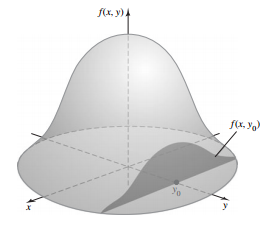
\includegraphics[width=0.4\linewidth]{fig/conditional_distribution.PNG}
\end{figure}
\begin{definition}[相互独立]
\[\begin{aligned}
F(x,y)=F_X(x)F_Y(y)\\
f(x,y)=f_X(x)f_Y(y)
\end{aligned}\]
\end{definition}

\subsection{随机变量的函数的分布}
均通过求$F_Z(z)=\pr{z\leq Z}$交换积分次序得到
\subsubsection{$Z=X+Y$}
\[f_{X+Y}(z)=\intabu{-\infty}{\infty}{f(z-y,y)}{y}=\intabu{-\infty}{\infty}{f(x,z-x)}{x}\]
\begin{analysis}
先求分布函数$F_Z(z)$
\[\begin{aligned}
F_Z(z)&=\pr{Z\leq z}=\iint_{x+y\leq z}f(x,y)\diff x\diff y\\
&=\int_{-\infty}^{+\infty}\int_{-\infty}^{z-y}f(x,y)\diff x\diff y\\
&=\int_{-\infty}^{+\infty}\int_{-\infty}^{z}f(u-y,y)\diff u\diff y\\
&=\int_{-\infty}^{z}\left[\int_{-\infty}^{+\infty}f(u-y,y)\diff y\right]\diff u
\end{aligned}\]
\end{analysis}
若$X$和$Y$相互独立,则有卷积公式
\[f_X*f_Y=\intabu{-\infty}{\infty}{f_X(z-y,y)f_Y(y)}{y}\]
\par 离散情形则有
\[f_{X+Y}(z)=\sum_{k=0}^zp(k)q(z-k),\,z=0,1,2,\ldots\]
\begin{example}
若$X,Y$相互独立,且$X\thicksim b(n_1,p),Y\thicksim b(n_2,p)$,证明$Z=X+Y\thicksim b(n_1+n_2,p)$
\end{example}
\begin{analysis}
\[\begin{aligned}
p(k)&=\binom{n_1}{k}p^k(1-p)^{n_1-k}\\
q(k)&=\binom{n_2}{k}p^k(1-p)^{n_2-k}\\
f(z)&=\sum_{k=0}^z\binom{n_1}{z}p^z(1-p)^{n_1-z}\binom{n_2}{z-k}p^{z-k}(1-p)^{z-n_2+k}\\
&=p^z(1-p)^{n_1+n_2-z}\sum_{k=0}^z\binom{n_1}{k}\binom{n_2}{z-k}\\
&=p^z(1-p)^{n_1+n_2-z}\binom{n_1+n_2}{z}\qquad\text{Vandermonde恒等式\footnote{* Vandermonde identity, \url{https://en.wikipedia.org/wiki/Vandermonde\%27s_identity}}}
\end{aligned}\]
\end{analysis}
\par 更一般地,$Z=a_1X_1+a_2X_2+b(a_1\ne 0)$,则$Y$有连续分布函数
\[g(y)=\int_{-\infty}^{+\infty}f\lrp{\frac{z-b-a_2x_2}{a_1},x_2}\frac{1}{|a_1|}\diff x_2\]

\subsubsection{$Z=Y/X$}
\[f_{Y/X}(z)=\intabu{-\infty}{\infty}{|x|f(x,xz)}{x}\]

\subsubsection{$Z=XY$}
\[f_{XY}(z)=\intinf{\dfrac{1}{|x|}f(x,\dfrac{z}{x})}\]

\subsubsection{$Z=\max\{X_1,\ldots,X_n\}$}
\[F_{\max}(z)=F_{X_1}(z)F_{X_2}(z)\cdots F_{X_n}(z)\]

\subsubsection{$Z=\min\{X_1,\ldots,X_n\}$}
\[F_{\min}(z)=1-[1-F_{X_1}(z)][1-F_{X_2}(z)]\cdots [1-F_{X_n}(z)]\]

\begin{example}
设随机变量$(X,Y)$的概率密度为
\[f(x,y)=\begin{cases}x+y&0<x<1,0<y<1\\0&\text{其他}\end{cases}\]
分别求$Z=X+Y$,$Z=XY$的概率密度
\end{example}
\begin{analysis}
关键在于求出相应的$f$在什么区间内有非零值!
\begin{enumerate}
	\item 由随机变量函数的分布有
	\[f_{X+Y}(z)=\int_{-\infty}^{+\infty}f(x,z-x)\diff x\]
	进而有范围,注意要确定积分限,关键看积分变量的范围
	\[\begin{cases}0<x<1\\0<z-x<1\end{cases}\implies\begin{cases}0<x<1\\z-1<x<z\end{cases}\]
	右式实际上是两个区间取交集,故分类讨论$z$的大小,得
	\[\begin{cases}z\in(0,1)&x\in(0,z)\\z\in[1,2)&x\in(z-1,1)\\z\notin(0,2)&x\in\varnothing\end{cases}\]
	在上述区间内$f(x,z-x)=z$,其余区间$f(x,z-x)=0$,故
	\[f_Z(z)=\begin{cases}\int_0^zz\diff x=z^2&z\in(0,1)\\\int_z^1z\diff x=2z-z^2&z\in[1,2)\\0&z\notin(0,2)\end{cases}\]
	\item 由随机变量函数的分布有
	\[f_{XY}(z)=\int_{-\infty}^{+\infty}\frac{1}{|x|}f\lrp{x,\frac{z}{x}}\diff x\]
	求积分限,注意这里$x$与$z$的正负关系,可将第一条式子作为前提,得到$z>0$
	\[\begin{cases}0<x<1\\0<\frac{z}{x}<1\end{cases}\implies\begin{cases}z\in(0,1)&x\in(z,1)\\z\notin(0,1)&x\in\varnothing\end{cases}\]
	故
	\[f_Z(z)=\begin{cases}\int_z^1\lrp{1+\frac{z}{x^2}}\diff x=2(1-z)&z\in(0,1)\\0&z\notin(0,1)\end{cases}\]
\end{enumerate}
\end{analysis}

\subsubsection{函数分布}
若$Z$是随机变量$X,Y$的连续函数$Z=g(X,Y)$,则
\[\E{Z}=\E{g(x,y)}=\intabu{-\infty}{\infty}{\intab{-\infty}{\infty}{g(x,y)f(x,y)}}{y}\]
根据这条式子,方差、协方差等等均可以直接通过积分计算

特别地,
\[\begin{aligned}
\E{X}&=\int_{-\infty}^\infty\int_{-\infty}^\infty xf(x,y)\diff x\diff y=\int_{-\infty}^\infty xf_X(x)\diff x\\
\E{Y}&=\int_{-\infty}^\infty\int_{-\infty}^\infty yf(x,y)\diff x\diff y=\int_{-\infty}^\infty yf_Y(y)\diff y\\
\E{XY}&=\int_{-\infty}^\infty\int_{-\infty}^\infty xyf(x,y)\diff x\diff y\\
\end{aligned}\]

\subsection{数字特征}
\begin{definition}[协方差]
\[\Cov{X,Y}=\E{[X-\E{X}][Y-\E{Y}]}=\E{XY}-\E{X}\E{Y}\]
协方差为$0$称为\textbf{不相关}
\end{definition}
协方差的性质:
\[\begin{aligned}
\Cov{aX,bY}&=ab\Cov{X,Y}\\
\Cov{X_1+X_2,Y}&=\Cov{X_1,Y}+\Cov{X_2,Y}
\end{aligned}\]
\begin{definition}[相关系数]
用来表征$X,Y$线性关系的量
\[\rho_{XY}=\frac{\Cov{X,Y}}{\sqrt{\Var{X}}\sqrt{\Var{Y}}}\]
$|\rho_{XY}|$较大,均方误差小,线性关系强;
$\rho_{XY}\leq 1$,取等的充要条件为$\exists a,b$使得$\pr{Y=a+bX}=1$
\end{definition}
相关性与独立性没有必然联系:相关性是对线性关系来说的,而独立性是对一般关系来说的
\begin{definition}[矩(moment)]
设$X,Y$为随机变量,若$\E{X^k}$存在,则称它为$X$的$k$阶(原点)矩,称$\E{[X-\E{X}]^k}$为$k$阶中心矩,称$\E{X^kY^l}$为$k+l$阶混合矩,称$\E{[X-\E{X}]^k[Y-\E{Y}]^l}$为$k+l$阶混合中心矩
\end{definition}
\begin{definition}[协方差矩阵]
设$n$维随机变量$(X_1,X_2,\ldots,X_n)$的二阶混合中心距
\[c_{ij}=\Cov{X_i,X_j}=\E{[X_i-\E{X_i}][X_j-\E{X_j}]}\]
都存在,则协方差矩阵
\[\mC=\begin{bmatrix}
c_{11}&c_{12}&\cdots&c_{1n}\\
c_{21}&c_{22}&\cdots&c_{2n}\\
\vdots&\vdots&\ddots&\vdots\\
c_{n1}&c_{n2}&\cdots&c_{nn}
\end{bmatrix}\]
又$c_{ij}=c_{ji}$,故上述矩阵是个对称矩阵
\end{definition}
\begin{theorem}
若$X_1,\ldots,X_n$独立,则
\[\begin{aligned}
\E{\prod_{i=1}^nX_i}&=\prod_{i=1}^n\E{X_i}\\
\Var{\prod_{i=1}^nX_i}&=\sum_{i=1}^n\Var{X_i}\\
\Cov{X_i,X_j}&=0,\,i\ne j
\end{aligned}\]
\end{theorem}
$Y=g(X)$的随机变量分布一般通过求分布函数后求导得到其概率密度函数